\documentclass[twoside]{book}

% Packages required by doxygen
\usepackage{fixltx2e}
\usepackage{calc}
\usepackage{doxygen}
\usepackage[export]{adjustbox} % also loads graphicx
\usepackage{graphicx}
\usepackage[utf8]{inputenc}
\usepackage{makeidx}
\usepackage{multicol}
\usepackage{multirow}
\PassOptionsToPackage{warn}{textcomp}
\usepackage{textcomp}
\usepackage[nointegrals]{wasysym}
\usepackage[table]{xcolor}

% Font selection
\usepackage[T1]{fontenc}
\usepackage[scaled=.90]{helvet}
\usepackage{courier}
\usepackage{amssymb}
\usepackage{sectsty}
\renewcommand{\familydefault}{\sfdefault}
\allsectionsfont{%
  \fontseries{bc}\selectfont%
  \color{darkgray}%
}
\renewcommand{\DoxyLabelFont}{%
  \fontseries{bc}\selectfont%
  \color{darkgray}%
}
\newcommand{\+}{\discretionary{\mbox{\scriptsize$\hookleftarrow$}}{}{}}

% Page & text layout
\usepackage{geometry}
\geometry{%
  a4paper,%
  top=2.5cm,%
  bottom=2.5cm,%
  left=2.5cm,%
  right=2.5cm%
}
\tolerance=750
\hfuzz=15pt
\hbadness=750
\setlength{\emergencystretch}{15pt}
\setlength{\parindent}{0cm}
\setlength{\parskip}{3ex plus 2ex minus 2ex}
\makeatletter
\renewcommand{\paragraph}{%
  \@startsection{paragraph}{4}{0ex}{-1.0ex}{1.0ex}{%
    \normalfont\normalsize\bfseries\SS@parafont%
  }%
}
\renewcommand{\subparagraph}{%
  \@startsection{subparagraph}{5}{0ex}{-1.0ex}{1.0ex}{%
    \normalfont\normalsize\bfseries\SS@subparafont%
  }%
}
\makeatother

% Headers & footers
\usepackage{fancyhdr}
\pagestyle{fancyplain}
\fancyhead[LE]{\fancyplain{}{\bfseries\thepage}}
\fancyhead[CE]{\fancyplain{}{}}
\fancyhead[RE]{\fancyplain{}{\bfseries\leftmark}}
\fancyhead[LO]{\fancyplain{}{\bfseries\rightmark}}
\fancyhead[CO]{\fancyplain{}{}}
\fancyhead[RO]{\fancyplain{}{\bfseries\thepage}}
\fancyfoot[LE]{\fancyplain{}{}}
\fancyfoot[CE]{\fancyplain{}{}}
\fancyfoot[RE]{\fancyplain{}{\bfseries\scriptsize Generated by Doxygen }}
\fancyfoot[LO]{\fancyplain{}{\bfseries\scriptsize Generated by Doxygen }}
\fancyfoot[CO]{\fancyplain{}{}}
\fancyfoot[RO]{\fancyplain{}{}}
\renewcommand{\footrulewidth}{0.4pt}
\renewcommand{\chaptermark}[1]{%
  \markboth{#1}{}%
}
\renewcommand{\sectionmark}[1]{%
  \markright{\thesection\ #1}%
}

% Indices & bibliography
\usepackage{natbib}
\usepackage[titles]{tocloft}
\setcounter{tocdepth}{3}
\setcounter{secnumdepth}{5}
\makeindex

% Hyperlinks (required, but should be loaded last)
\usepackage{ifpdf}
\ifpdf
  \usepackage[pdftex,pagebackref=true]{hyperref}
\else
  \usepackage[ps2pdf,pagebackref=true]{hyperref}
\fi
\hypersetup{%
  colorlinks=true,%
  linkcolor=blue,%
  citecolor=blue,%
  unicode%
}

% Custom commands
\newcommand{\clearemptydoublepage}{%
  \newpage{\pagestyle{empty}\cleardoublepage}%
}

\usepackage{caption}
\captionsetup{labelsep=space,justification=centering,font={bf},singlelinecheck=off,skip=4pt,position=top}

%===== C O N T E N T S =====

\begin{document}

% Titlepage & ToC
\hypersetup{pageanchor=false,
             bookmarksnumbered=true,
             pdfencoding=unicode
            }
\pagenumbering{alph}
\begin{titlepage}
\vspace*{7cm}
\begin{center}%
{\Large n\+Gram search \\[1ex]\large 1.\+0 }\\
\vspace*{1cm}
{\large Generated by Doxygen 1.8.14}\\
\end{center}
\end{titlepage}
\clearemptydoublepage
\pagenumbering{roman}
\tableofcontents
\clearemptydoublepage
\pagenumbering{arabic}
\hypersetup{pageanchor=true}

%--- Begin generated contents ---
\chapter{Class Index}
\section{Class List}
Here are the classes, structs, unions and interfaces with brief descriptions\+:\begin{DoxyCompactList}
\item\contentsline{section}{\mbox{\hyperlink{class_string_index}{String\+Index$<$ str\+\_\+t $>$}} }{\pageref{class_string_index}}{}
\end{DoxyCompactList}

\chapter{Class Documentation}
\hypertarget{class_string_index}{}\section{String\+Index$<$ str\+\_\+t $>$ Class Template Reference}
\label{class_string_index}\index{String\+Index$<$ str\+\_\+t $>$@{String\+Index$<$ str\+\_\+t $>$}}


{\ttfamily \#include $<$n\+Gram\+Search.\+h$>$}

\subsection*{Public Types}
\begin{DoxyCompactItemize}
\item 
\mbox{\Hypertarget{class_string_index_a47f131c73d15a7c10c10a9748adf45dc}\label{class_string_index_a47f131c73d15a7c10c10a9748adf45dc}} 
typedef str\+\_\+t\+::value\+\_\+type \mbox{\hyperlink{class_string_index_a47f131c73d15a7c10c10a9748adf45dc}{char\+\_\+t}}
\begin{DoxyCompactList}\small\item\em The character type invelved in the str\+\_\+t. \end{DoxyCompactList}\end{DoxyCompactItemize}
\subsection*{Public Member Functions}
\begin{DoxyCompactItemize}
\item 
\mbox{\hyperlink{class_string_index_aec0c7112ef81d953265033f9a779730f}{String\+Index}} (\mbox{\hyperlink{class_string_index_a47f131c73d15a7c10c10a9748adf45dc}{char\+\_\+t}} $\ast$$\ast$const words, const size\+\_\+t \mbox{\hyperlink{class_string_index_a95acf789f43ead39b067d1c82d3a9b02}{size}}, const uint16\+\_\+t row\+Size, float $\ast$const weight, const uint16\+\_\+t g\+Size)
\item 
\mbox{\hyperlink{class_string_index_a2e323737994e475a5e5b6ccc9f631fff}{String\+Index}} (\mbox{\hyperlink{class_string_index_a47f131c73d15a7c10c10a9748adf45dc}{char\+\_\+t}} $\ast$$\ast$$\ast$const words, const size\+\_\+t \mbox{\hyperlink{class_string_index_a95acf789f43ead39b067d1c82d3a9b02}{size}}, const uint16\+\_\+t row\+Size, float $\ast$$\ast$const weight, const uint16\+\_\+t g\+Size)
\item 
\mbox{\hyperlink{class_string_index_ab7114eb0acf9e736de851487398a4cef}{String\+Index}} (std\+::vector$<$ std\+::vector$<$ str\+\_\+t $>$$>$ \&words, const int16\+\_\+t g\+Size, std\+::vector$<$ std\+::vector$<$ float $>$$>$ \&weight)
\item 
void \mbox{\hyperlink{class_string_index_a56c849706990da23bb621522da959fa9}{init}} (std\+::unordered\+\_\+map$<$ str\+\_\+t, std\+::vector$<$ std\+::pair$<$ str\+\_\+t, float $>$$>$$>$ \&temp\+Word\+Map)
\item 
void \mbox{\hyperlink{class_string_index_a924cd52b4e055853db22f89e73f71fce}{get\+Grams}} (str\+\_\+t $\ast$str)
\item 
void \mbox{\hyperlink{class_string_index_a1b66797dae7f0f1d4f3cf830dfeee869}{get\+Grams}} (const str\+\_\+t \&str, std\+::vector$<$ str\+\_\+t $>$ \&generated\+Grams)
\item 
void \mbox{\hyperlink{class_string_index_a7e326eb6fe367a6758c21aefbf64fe51}{build\+Grams}} ()
\item 
size\+\_\+t \mbox{\hyperlink{class_string_index_a97835599308c1e5feb47323545584dfd}{string\+Match}} (const str\+\_\+t \&query, const str\+\_\+t \&source, std\+::vector$<$ size\+\_\+t $>$ \&row1, std\+::vector$<$ size\+\_\+t $>$ \&row2)
\item 
void \mbox{\hyperlink{class_string_index_a32f2294a19ad5360bd62f1ede07c6c5e}{get\+Match\+Score}} (const str\+\_\+t \&query, size\+\_\+t first, std\+::vector$<$ str\+\_\+t $\ast$$>$ \&targets, std\+::vector$<$ float $>$ \&current\+Score)
\item 
void \mbox{\hyperlink{class_string_index_a309f7697439fb3428de3c63dca6cdaa4}{search\+Short}} (str\+\_\+t \&query, std\+::unordered\+\_\+map$<$ str\+\_\+t $\ast$, float $>$ \&score)
\item 
void \mbox{\hyperlink{class_string_index_a80ddf83f3f207004142458317609c6d6}{search\+Long}} (str\+\_\+t \&query, std\+::unordered\+\_\+map$<$ str\+\_\+t $\ast$, float $>$ \&score)
\item 
void \mbox{\hyperlink{class_string_index_adedd1463c2745dcd1e36ee672f6a6613}{\+\_\+search}} (const \mbox{\hyperlink{class_string_index_a47f131c73d15a7c10c10a9748adf45dc}{char\+\_\+t}} $\ast$query, const float threshold, const uint32\+\_\+t limit, std\+::vector$<$ str\+\_\+t $>$ \&result)
\item 
void \mbox{\hyperlink{class_string_index_aa11036396dce714b8c383564ffeaac70}{search}} (const \mbox{\hyperlink{class_string_index_a47f131c73d15a7c10c10a9748adf45dc}{char\+\_\+t}} $\ast$query, \mbox{\hyperlink{class_string_index_a47f131c73d15a7c10c10a9748adf45dc}{char\+\_\+t}} $\ast$$\ast$$\ast$results, uint32\+\_\+t $\ast$\mbox{\hyperlink{class_string_index_a95acf789f43ead39b067d1c82d3a9b02}{size}}, const float threshold, uint32\+\_\+t limit)
\item 
void \mbox{\hyperlink{class_string_index_a014f9cc45c6e06aa25b04186c89ec032}{release}} (\mbox{\hyperlink{class_string_index_a47f131c73d15a7c10c10a9748adf45dc}{char\+\_\+t}} $\ast$$\ast$$\ast$results, size\+\_\+t \mbox{\hyperlink{class_string_index_a95acf789f43ead39b067d1c82d3a9b02}{size}}) const
\item 
uint64\+\_\+t \mbox{\hyperlink{class_string_index_a95acf789f43ead39b067d1c82d3a9b02}{size}} ()
\item 
uint64\+\_\+t \mbox{\hyperlink{class_string_index_af92d29d09732cbf9104cc7e942859976}{lib\+Size}} ()
\end{DoxyCompactItemize}
\subsection*{Static Public Member Functions}
\begin{DoxyCompactItemize}
\item 
{\footnotesize template$<$class str\+\_\+t $>$ }\\static bool \mbox{\hyperlink{class_string_index_ab9646ee784190f04dba8d1e245c6be18}{compare\+Scores}} (std\+::pair$<$ str\+\_\+t, float $>$ \&a, std\+::pair$<$ str\+\_\+t, float $>$ \&b)
\item 
{\footnotesize template$<$class str\+\_\+t $>$ }\\static void \mbox{\hyperlink{class_string_index_ac75c72953237b8361e7f35fe952657c4}{trim}} (str\+\_\+t \&s)
\end{DoxyCompactItemize}
\subsection*{Protected Attributes}
\begin{DoxyCompactItemize}
\item 
\mbox{\Hypertarget{class_string_index_ac41713b30c0c373a3e9fc3efe13f9949}\label{class_string_index_ac41713b30c0c373a3e9fc3efe13f9949}} 
std\+::vector$<$ str\+\_\+t $>$ \mbox{\hyperlink{class_string_index_ac41713b30c0c373a3e9fc3efe13f9949}{long\+Lib}}
\begin{DoxyCompactList}\small\item\em The library for all words that have a length $>$= {\ttfamily gram\+Size} $\ast$ 2. \end{DoxyCompactList}\item 
\mbox{\Hypertarget{class_string_index_a4f0c00d4ace341b657ac1b233b70534b}\label{class_string_index_a4f0c00d4ace341b657ac1b233b70534b}} 
std\+::vector$<$ str\+\_\+t $>$ \mbox{\hyperlink{class_string_index_a4f0c00d4ace341b657ac1b233b70534b}{short\+Lib}}
\begin{DoxyCompactList}\small\item\em The library for all words that have a length $<$ {\ttfamily gram\+Size} $\ast$ 2. \end{DoxyCompactList}\item 
\mbox{\Hypertarget{class_string_index_aaf98238698a0294638fb474c4962eac7}\label{class_string_index_aaf98238698a0294638fb474c4962eac7}} 
std\+::unordered\+\_\+map$<$ str\+\_\+t $\ast$, std\+::vector$<$ std\+::pair$<$ str\+\_\+t, float $>$ $>$ $>$ \mbox{\hyperlink{class_string_index_aaf98238698a0294638fb474c4962eac7}{word\+Map}}
\begin{DoxyCompactList}\small\item\em All words, mapped to their master keys. A search result will always be redirected to its master keys. \end{DoxyCompactList}\item 
\mbox{\Hypertarget{class_string_index_adae09412441dcac487fd942660ca72f5}\label{class_string_index_adae09412441dcac487fd942660ca72f5}} 
std\+::unordered\+\_\+map$<$ str\+\_\+t, std\+::unordered\+\_\+set$<$ str\+\_\+t $\ast$ $>$ $>$ \mbox{\hyperlink{class_string_index_adae09412441dcac487fd942660ca72f5}{ngrams}}
\begin{DoxyCompactList}\small\item\em The n-\/gram library generated. \end{DoxyCompactList}\item 
\mbox{\Hypertarget{class_string_index_aadcaf2dd0a288b18d85febf8157de6be}\label{class_string_index_aadcaf2dd0a288b18d85febf8157de6be}} 
int16\+\_\+t \mbox{\hyperlink{class_string_index_aadcaf2dd0a288b18d85febf8157de6be}{gram\+Size}} = 3
\begin{DoxyCompactList}\small\item\em the size of n-\/grams \end{DoxyCompactList}\end{DoxyCompactItemize}


\subsection{Detailed Description}
\subsubsection*{template$<$class str\+\_\+t$>$\newline
class String\+Index$<$ str\+\_\+t $>$}

\mbox{\hyperlink{class_string_index}{String\+Index}}\+: Each instance manages a library from the $<$index$>$ function 
\begin{DoxyParams}{Parameters}
{\em str\+\_\+t} & A S\+TL string type. Can be std\+::string or std\+::wstring \\
\hline
\end{DoxyParams}


\subsection{Constructor \& Destructor Documentation}
\mbox{\Hypertarget{class_string_index_aec0c7112ef81d953265033f9a779730f}\label{class_string_index_aec0c7112ef81d953265033f9a779730f}} 
\index{String\+Index@{String\+Index}!String\+Index@{String\+Index}}
\index{String\+Index@{String\+Index}!String\+Index@{String\+Index}}
\subsubsection{\texorpdfstring{String\+Index()}{StringIndex()}\hspace{0.1cm}{\footnotesize\ttfamily [1/3]}}
{\footnotesize\ttfamily template$<$class str\+\_\+t $>$ \\
\mbox{\hyperlink{class_string_index}{String\+Index}}$<$ str\+\_\+t $>$\+::\mbox{\hyperlink{class_string_index}{String\+Index}} (\begin{DoxyParamCaption}\item[{\mbox{\hyperlink{class_string_index_a47f131c73d15a7c10c10a9748adf45dc}{char\+\_\+t}} $\ast$$\ast$const}]{words,  }\item[{const size\+\_\+t}]{size,  }\item[{const uint16\+\_\+t}]{row\+Size,  }\item[{float $\ast$const}]{weight,  }\item[{const uint16\+\_\+t}]{g\+Size }\end{DoxyParamCaption})}

Constructs the \mbox{\hyperlink{class_string_index}{String\+Index}} class by indexing the strings based on an array of words 
\begin{DoxyParams}{Parameters}
{\em words} & Words to be searched for. For each row, the first word is used as the master key, in which the row size is {\ttfamily row\+Size}. All rows are flattened into a 1\+D-\/array, and can be extracted based on {\ttfamily row\+Size}. In a search, all queries of the words in a row will return the master key. \\
\hline
{\em size} & size of the {\ttfamily words} \\
\hline
{\em row\+Size} & size of each text rows of {\ttfamily words}. \\
\hline
{\em weight} & A list of weight values for each key. It should be at least as long as the number of rows, i.\+e. {\ttfamily size} / {\ttfamily row\+Size}. \\
\hline
{\em g\+Size} & size of grams to be created. Default 3. \\
\hline
\end{DoxyParams}
\mbox{\Hypertarget{class_string_index_a2e323737994e475a5e5b6ccc9f631fff}\label{class_string_index_a2e323737994e475a5e5b6ccc9f631fff}} 
\index{String\+Index@{String\+Index}!String\+Index@{String\+Index}}
\index{String\+Index@{String\+Index}!String\+Index@{String\+Index}}
\subsubsection{\texorpdfstring{String\+Index()}{StringIndex()}\hspace{0.1cm}{\footnotesize\ttfamily [2/3]}}
{\footnotesize\ttfamily template$<$class str\+\_\+t $>$ \\
\mbox{\hyperlink{class_string_index}{String\+Index}}$<$ str\+\_\+t $>$\+::\mbox{\hyperlink{class_string_index}{String\+Index}} (\begin{DoxyParamCaption}\item[{\mbox{\hyperlink{class_string_index_a47f131c73d15a7c10c10a9748adf45dc}{char\+\_\+t}} $\ast$$\ast$$\ast$const}]{words,  }\item[{const size\+\_\+t}]{size,  }\item[{const uint16\+\_\+t}]{row\+Size,  }\item[{float $\ast$$\ast$const}]{weight,  }\item[{const uint16\+\_\+t}]{g\+Size }\end{DoxyParamCaption})}

Constructs the \mbox{\hyperlink{class_string_index}{String\+Index}} class by indexing the strings based on an array of words 
\begin{DoxyParams}{Parameters}
{\em words} & Words to be searched for. For each row, the first word is used as the master key, in which the row size is {\ttfamily row\+Size}. Each row is in a separate sub-\/array. In a search, all queries of the words in a row will return the master key. \\
\hline
{\em size} & size of the {\ttfamily words} \\
\hline
{\em row\+Size} & size of each text rows of {\ttfamily words}. \\
\hline
{\em weight} & A list of weight values for each key. It should be at least as long as the number of rows, i.\+e. {\ttfamily size} / {\ttfamily row\+Size}. \\
\hline
{\em g\+Size} & size of grams to be created. Default 3. \\
\hline
\end{DoxyParams}
\mbox{\Hypertarget{class_string_index_ab7114eb0acf9e736de851487398a4cef}\label{class_string_index_ab7114eb0acf9e736de851487398a4cef}} 
\index{String\+Index@{String\+Index}!String\+Index@{String\+Index}}
\index{String\+Index@{String\+Index}!String\+Index@{String\+Index}}
\subsubsection{\texorpdfstring{String\+Index()}{StringIndex()}\hspace{0.1cm}{\footnotesize\ttfamily [3/3]}}
{\footnotesize\ttfamily template$<$class str\+\_\+t $>$ \\
\mbox{\hyperlink{class_string_index}{String\+Index}}$<$ str\+\_\+t $>$\+::\mbox{\hyperlink{class_string_index}{String\+Index}} (\begin{DoxyParamCaption}\item[{std\+::vector$<$ std\+::vector$<$ str\+\_\+t $>$$>$ \&}]{words,  }\item[{const int16\+\_\+t}]{g\+Size,  }\item[{std\+::vector$<$ std\+::vector$<$ float $>$$>$ \&}]{weight }\end{DoxyParamCaption})}

Constructs the \mbox{\hyperlink{class_string_index}{String\+Index}} class by indexing the strings based on an array of words 
\begin{DoxyParams}{Parameters}
{\em words} & Words to be searched for. For each row, the first word is used as the master key, in which the row size is {\ttfamily row\+Size}. Each row is in a separate sub-\/array. In a search, all queries of the words in a row will return the master key. \\
\hline
{\em size} & size of the {\ttfamily words} \\
\hline
{\em row\+Size} & size of each text rows of {\ttfamily words}. \\
\hline
{\em weight} & A list of weight values for each key. It should be at least as long as the number of rows, i.\+e. {\ttfamily size} / {\ttfamily row\+Size}. \\
\hline
{\em g\+Size} & size of grams to be created. Default 3. \\
\hline
\end{DoxyParams}


\subsection{Member Function Documentation}
\mbox{\Hypertarget{class_string_index_adedd1463c2745dcd1e36ee672f6a6613}\label{class_string_index_adedd1463c2745dcd1e36ee672f6a6613}} 
\index{String\+Index@{String\+Index}!\+\_\+search@{\+\_\+search}}
\index{\+\_\+search@{\+\_\+search}!String\+Index@{String\+Index}}
\subsubsection{\texorpdfstring{\+\_\+search()}{\_search()}}
{\footnotesize\ttfamily template$<$class str\+\_\+t $>$ \\
void \mbox{\hyperlink{class_string_index}{String\+Index}}$<$ str\+\_\+t $>$\+::\+\_\+search (\begin{DoxyParamCaption}\item[{const \mbox{\hyperlink{class_string_index_a47f131c73d15a7c10c10a9748adf45dc}{char\+\_\+t}} $\ast$}]{query,  }\item[{const float}]{threshold,  }\item[{const uint32\+\_\+t}]{limit,  }\item[{std\+::vector$<$ str\+\_\+t $>$ \&}]{result }\end{DoxyParamCaption})}

The worker function for search 
\begin{DoxyParams}{Parameters}
{\em query} & The query string. \\
\hline
{\em threshold} & Lowest acceptable match ratio for a string to be included in the results. \\
\hline
{\em limit} & The maximum number of results to generate. \\
\hline
{\em result} & The matching strings to be selected, sorted from highest score to lowest. \\
\hline
\end{DoxyParams}
Here is the call graph for this function\+:\nopagebreak
\begin{figure}[H]
\begin{center}
\leavevmode
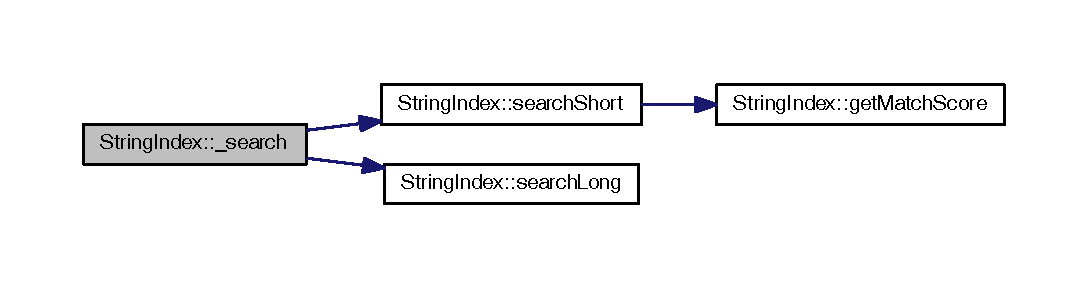
\includegraphics[width=350pt]{class_string_index_adedd1463c2745dcd1e36ee672f6a6613_cgraph}
\end{center}
\end{figure}
\mbox{\Hypertarget{class_string_index_a7e326eb6fe367a6758c21aefbf64fe51}\label{class_string_index_a7e326eb6fe367a6758c21aefbf64fe51}} 
\index{String\+Index@{String\+Index}!build\+Grams@{build\+Grams}}
\index{build\+Grams@{build\+Grams}!String\+Index@{String\+Index}}
\subsubsection{\texorpdfstring{build\+Grams()}{buildGrams()}}
{\footnotesize\ttfamily template$<$class str\+\_\+t $>$ \\
void \mbox{\hyperlink{class_string_index}{String\+Index}}$<$ str\+\_\+t $>$\+::build\+Grams (\begin{DoxyParamCaption}{ }\end{DoxyParamCaption})}

Build n-\/grams for the member variable {\ttfamily long\+Lib} \mbox{\Hypertarget{class_string_index_ab9646ee784190f04dba8d1e245c6be18}\label{class_string_index_ab9646ee784190f04dba8d1e245c6be18}} 
\index{String\+Index@{String\+Index}!compare\+Scores@{compare\+Scores}}
\index{compare\+Scores@{compare\+Scores}!String\+Index@{String\+Index}}
\subsubsection{\texorpdfstring{compare\+Scores()}{compareScores()}}
{\footnotesize\ttfamily template$<$class str\+\_\+t $>$ \\
template$<$class str\+\_\+t $>$ \\
static bool \mbox{\hyperlink{class_string_index}{String\+Index}}$<$ str\+\_\+t $>$\+::compare\+Scores (\begin{DoxyParamCaption}\item[{std\+::pair$<$ str\+\_\+t, float $>$ \&}]{a,  }\item[{std\+::pair$<$ str\+\_\+t, float $>$ \&}]{b }\end{DoxyParamCaption})\hspace{0.3cm}{\ttfamily [inline]}, {\ttfamily [static]}}

Compare pairs of string-\/score by their score, and length. Greater scores and shorter lengths will be prioritized 
\begin{DoxyParams}{Parameters}
{\em a} & The first pair of string-\/score \\
\hline
{\em b} & The second pair of string-\/score \\
\hline
\end{DoxyParams}
\mbox{\Hypertarget{class_string_index_a924cd52b4e055853db22f89e73f71fce}\label{class_string_index_a924cd52b4e055853db22f89e73f71fce}} 
\index{String\+Index@{String\+Index}!get\+Grams@{get\+Grams}}
\index{get\+Grams@{get\+Grams}!String\+Index@{String\+Index}}
\subsubsection{\texorpdfstring{get\+Grams()}{getGrams()}\hspace{0.1cm}{\footnotesize\ttfamily [1/2]}}
{\footnotesize\ttfamily template$<$class str\+\_\+t $>$ \\
void \mbox{\hyperlink{class_string_index}{String\+Index}}$<$ str\+\_\+t $>$\+::get\+Grams (\begin{DoxyParamCaption}\item[{str\+\_\+t $\ast$}]{str }\end{DoxyParamCaption})}

Generate n-\/grams from a string based on the member variable {\ttfamily gram\+Size}. 
\begin{DoxyParams}{Parameters}
{\em str} & A pointer to the string to generate n-\/grams from. \\
\hline
\end{DoxyParams}
\mbox{\Hypertarget{class_string_index_a1b66797dae7f0f1d4f3cf830dfeee869}\label{class_string_index_a1b66797dae7f0f1d4f3cf830dfeee869}} 
\index{String\+Index@{String\+Index}!get\+Grams@{get\+Grams}}
\index{get\+Grams@{get\+Grams}!String\+Index@{String\+Index}}
\subsubsection{\texorpdfstring{get\+Grams()}{getGrams()}\hspace{0.1cm}{\footnotesize\ttfamily [2/2]}}
{\footnotesize\ttfamily template$<$class str\+\_\+t $>$ \\
void \mbox{\hyperlink{class_string_index}{String\+Index}}$<$ str\+\_\+t $>$\+::get\+Grams (\begin{DoxyParamCaption}\item[{const str\+\_\+t \&}]{str,  }\item[{std\+::vector$<$ str\+\_\+t $>$ \&}]{generated\+Grams }\end{DoxyParamCaption})}

Generate n-\/grams from a string based on the member variable {\ttfamily gram\+Size}, and store in an array. 
\begin{DoxyParams}{Parameters}
{\em str} & A pointer to the string to generate n-\/grams from. \\
\hline
{\em generated\+Grams} & A vector to store the genearated n-\/grams \\
\hline
\end{DoxyParams}
\mbox{\Hypertarget{class_string_index_a32f2294a19ad5360bd62f1ede07c6c5e}\label{class_string_index_a32f2294a19ad5360bd62f1ede07c6c5e}} 
\index{String\+Index@{String\+Index}!get\+Match\+Score@{get\+Match\+Score}}
\index{get\+Match\+Score@{get\+Match\+Score}!String\+Index@{String\+Index}}
\subsubsection{\texorpdfstring{get\+Match\+Score()}{getMatchScore()}}
{\footnotesize\ttfamily template$<$class str\+\_\+t $>$ \\
void \mbox{\hyperlink{class_string_index}{String\+Index}}$<$ str\+\_\+t $>$\+::get\+Match\+Score (\begin{DoxyParamCaption}\item[{const str\+\_\+t \&}]{query,  }\item[{size\+\_\+t}]{first,  }\item[{std\+::vector$<$ str\+\_\+t $\ast$$>$ \&}]{targets,  }\item[{std\+::vector$<$ float $>$ \&}]{current\+Score }\end{DoxyParamCaption})}

A looper to calculate match scores 
\begin{DoxyParams}{Parameters}
{\em query} & The query string. \\
\hline
{\em first} & The starting index to loop from. \\
\hline
{\em targets} & The target strings that have been scored \\
\hline
{\em current\+Score} & The score for each strings in {\ttfamily targets} \\
\hline
\end{DoxyParams}
Here is the caller graph for this function\+:\nopagebreak
\begin{figure}[H]
\begin{center}
\leavevmode
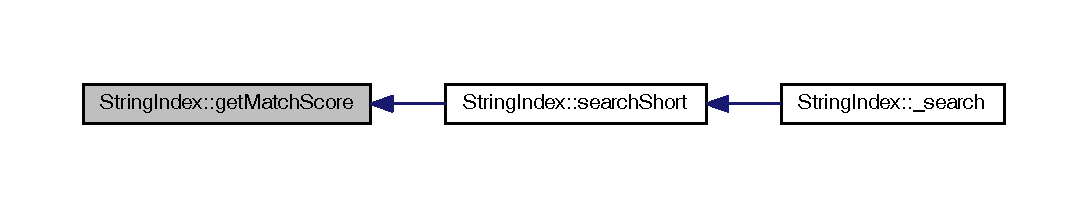
\includegraphics[width=350pt]{class_string_index_a32f2294a19ad5360bd62f1ede07c6c5e_icgraph}
\end{center}
\end{figure}
\mbox{\Hypertarget{class_string_index_a56c849706990da23bb621522da959fa9}\label{class_string_index_a56c849706990da23bb621522da959fa9}} 
\index{String\+Index@{String\+Index}!init@{init}}
\index{init@{init}!String\+Index@{String\+Index}}
\subsubsection{\texorpdfstring{init()}{init()}}
{\footnotesize\ttfamily template$<$class str\+\_\+t $>$ \\
void \mbox{\hyperlink{class_string_index}{String\+Index}}$<$ str\+\_\+t $>$\+::init (\begin{DoxyParamCaption}\item[{std\+::unordered\+\_\+map$<$ str\+\_\+t, std\+::vector$<$ std\+::pair$<$ str\+\_\+t, float $>$$>$$>$ \&}]{temp\+Word\+Map }\end{DoxyParamCaption})}

Initiates the word map by assigning the same strings to a pointer, to save space. 
\begin{DoxyParams}{Parameters}
{\em temp\+Word\+Map} & A temprary word map of strings. Key\+: query terms. Value\+: a list of master keys and corresponding scores that the queries point to. \\
\hline
\end{DoxyParams}
\mbox{\Hypertarget{class_string_index_af92d29d09732cbf9104cc7e942859976}\label{class_string_index_af92d29d09732cbf9104cc7e942859976}} 
\index{String\+Index@{String\+Index}!lib\+Size@{lib\+Size}}
\index{lib\+Size@{lib\+Size}!String\+Index@{String\+Index}}
\subsubsection{\texorpdfstring{lib\+Size()}{libSize()}}
{\footnotesize\ttfamily template$<$class str\+\_\+t $>$ \\
uint64\+\_\+t \mbox{\hyperlink{class_string_index}{String\+Index}}$<$ str\+\_\+t $>$\+::lib\+Size (\begin{DoxyParamCaption}{ }\end{DoxyParamCaption})}

Get the size of the n-\/gram library {\ttfamily ngrams} \mbox{\Hypertarget{class_string_index_a014f9cc45c6e06aa25b04186c89ec032}\label{class_string_index_a014f9cc45c6e06aa25b04186c89ec032}} 
\index{String\+Index@{String\+Index}!release@{release}}
\index{release@{release}!String\+Index@{String\+Index}}
\subsubsection{\texorpdfstring{release()}{release()}}
{\footnotesize\ttfamily template$<$class str\+\_\+t $>$ \\
void \mbox{\hyperlink{class_string_index}{String\+Index}}$<$ str\+\_\+t $>$\+::release (\begin{DoxyParamCaption}\item[{\mbox{\hyperlink{class_string_index_a47f131c73d15a7c10c10a9748adf45dc}{char\+\_\+t}} $\ast$$\ast$$\ast$}]{results,  }\item[{size\+\_\+t}]{size }\end{DoxyParamCaption}) const}

Release a result pointer that have been generated in {\ttfamily search} 
\begin{DoxyParams}{Parameters}
{\em results} & The matching strings to be selected, allocated using the {\ttfamily new} operator. \\
\hline
\end{DoxyParams}
\mbox{\Hypertarget{class_string_index_aa11036396dce714b8c383564ffeaac70}\label{class_string_index_aa11036396dce714b8c383564ffeaac70}} 
\index{String\+Index@{String\+Index}!search@{search}}
\index{search@{search}!String\+Index@{String\+Index}}
\subsubsection{\texorpdfstring{search()}{search()}}
{\footnotesize\ttfamily template$<$class str\+\_\+t $>$ \\
void \mbox{\hyperlink{class_string_index}{String\+Index}}$<$ str\+\_\+t $>$\+::search (\begin{DoxyParamCaption}\item[{const \mbox{\hyperlink{class_string_index_a47f131c73d15a7c10c10a9748adf45dc}{char\+\_\+t}} $\ast$}]{query,  }\item[{\mbox{\hyperlink{class_string_index_a47f131c73d15a7c10c10a9748adf45dc}{char\+\_\+t}} $\ast$$\ast$$\ast$}]{results,  }\item[{uint32\+\_\+t $\ast$}]{size,  }\item[{const float}]{threshold,  }\item[{uint32\+\_\+t}]{limit }\end{DoxyParamCaption})}

The search interface function, calls {\ttfamily \+\_\+search} 
\begin{DoxyParams}{Parameters}
{\em query} & The query string. \\
\hline
{\em results} & The matching strings to be selected, sorted from highest score to lowest. \\
\hline
{\em size} & The number of strings in the result array. \\
\hline
{\em threshold} & Lowest acceptable match ratio for a string to be included in the results. \\
\hline
{\em limit} & The maximum number of results to generate. \\
\hline
\end{DoxyParams}
\mbox{\Hypertarget{class_string_index_a80ddf83f3f207004142458317609c6d6}\label{class_string_index_a80ddf83f3f207004142458317609c6d6}} 
\index{String\+Index@{String\+Index}!search\+Long@{search\+Long}}
\index{search\+Long@{search\+Long}!String\+Index@{String\+Index}}
\subsubsection{\texorpdfstring{search\+Long()}{searchLong()}}
{\footnotesize\ttfamily template$<$class str\+\_\+t $>$ \\
void \mbox{\hyperlink{class_string_index}{String\+Index}}$<$ str\+\_\+t $>$\+::search\+Long (\begin{DoxyParamCaption}\item[{str\+\_\+t \&}]{query,  }\item[{std\+::unordered\+\_\+map$<$ str\+\_\+t $\ast$, float $>$ \&}]{score }\end{DoxyParamCaption})}

Search in the long\+Lib 
\begin{DoxyParams}{Parameters}
{\em query} & The query string. \\
\hline
{\em score} & Targets found paired with their corresponding cores generated. \\
\hline
\end{DoxyParams}
Here is the caller graph for this function\+:\nopagebreak
\begin{figure}[H]
\begin{center}
\leavevmode
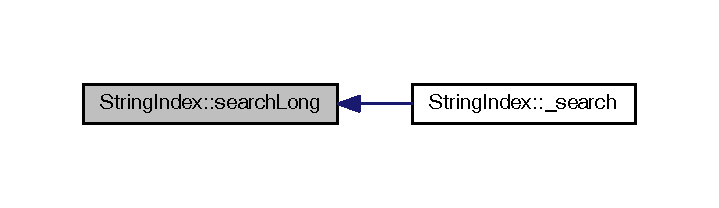
\includegraphics[width=345pt]{class_string_index_a80ddf83f3f207004142458317609c6d6_icgraph}
\end{center}
\end{figure}
\mbox{\Hypertarget{class_string_index_a309f7697439fb3428de3c63dca6cdaa4}\label{class_string_index_a309f7697439fb3428de3c63dca6cdaa4}} 
\index{String\+Index@{String\+Index}!search\+Short@{search\+Short}}
\index{search\+Short@{search\+Short}!String\+Index@{String\+Index}}
\subsubsection{\texorpdfstring{search\+Short()}{searchShort()}}
{\footnotesize\ttfamily template$<$class str\+\_\+t $>$ \\
void \mbox{\hyperlink{class_string_index}{String\+Index}}$<$ str\+\_\+t $>$\+::search\+Short (\begin{DoxyParamCaption}\item[{str\+\_\+t \&}]{query,  }\item[{std\+::unordered\+\_\+map$<$ str\+\_\+t $\ast$, float $>$ \&}]{score }\end{DoxyParamCaption})}

Search in the short\+Lib 
\begin{DoxyParams}{Parameters}
{\em query} & The query string. \\
\hline
{\em score} & Targets found paired with their corresponding cores generated. \\
\hline
\end{DoxyParams}
Here is the call graph for this function\+:\nopagebreak
\begin{figure}[H]
\begin{center}
\leavevmode
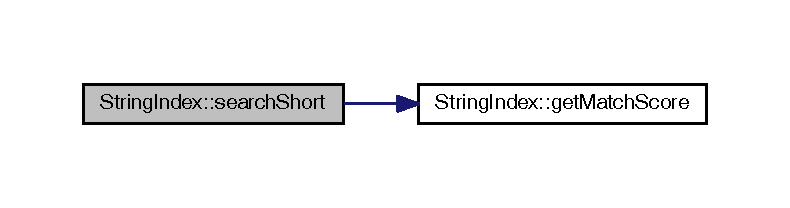
\includegraphics[width=350pt]{class_string_index_a309f7697439fb3428de3c63dca6cdaa4_cgraph}
\end{center}
\end{figure}
Here is the caller graph for this function\+:\nopagebreak
\begin{figure}[H]
\begin{center}
\leavevmode
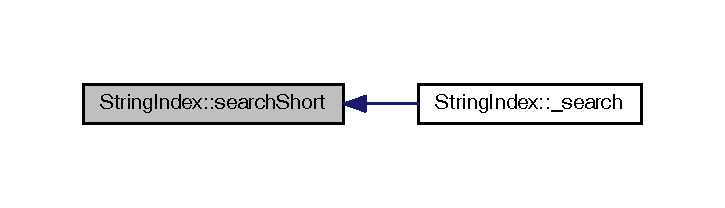
\includegraphics[width=348pt]{class_string_index_a309f7697439fb3428de3c63dca6cdaa4_icgraph}
\end{center}
\end{figure}
\mbox{\Hypertarget{class_string_index_a95acf789f43ead39b067d1c82d3a9b02}\label{class_string_index_a95acf789f43ead39b067d1c82d3a9b02}} 
\index{String\+Index@{String\+Index}!size@{size}}
\index{size@{size}!String\+Index@{String\+Index}}
\subsubsection{\texorpdfstring{size()}{size()}}
{\footnotesize\ttfamily template$<$class str\+\_\+t $>$ \\
uint64\+\_\+t \mbox{\hyperlink{class_string_index}{String\+Index}}$<$ str\+\_\+t $>$\+::size (\begin{DoxyParamCaption}{ }\end{DoxyParamCaption})}

Get the size of the word map {\ttfamily word\+Map} \mbox{\Hypertarget{class_string_index_a97835599308c1e5feb47323545584dfd}\label{class_string_index_a97835599308c1e5feb47323545584dfd}} 
\index{String\+Index@{String\+Index}!string\+Match@{string\+Match}}
\index{string\+Match@{string\+Match}!String\+Index@{String\+Index}}
\subsubsection{\texorpdfstring{string\+Match()}{stringMatch()}}
{\footnotesize\ttfamily template$<$class str\+\_\+t $>$ \\
size\+\_\+t \mbox{\hyperlink{class_string_index}{String\+Index}}$<$ str\+\_\+t $>$\+::string\+Match (\begin{DoxyParamCaption}\item[{const str\+\_\+t \&}]{query,  }\item[{const str\+\_\+t \&}]{source,  }\item[{std\+::vector$<$ size\+\_\+t $>$ \&}]{row1,  }\item[{std\+::vector$<$ size\+\_\+t $>$ \&}]{row2 }\end{DoxyParamCaption})}

Computes the percentage of {\ttfamily query} matches {\ttfamily source}. 
\begin{DoxyParams}{Parameters}
{\em query} & A query string \\
\hline
{\em source} & A source string in the library to compare to. \\
\hline
{\em row1} & A temporary vector as a cache for the algorithm. Its size must at least (the max size of {\ttfamily query} and {\ttfamily source}) + 1. \\
\hline
{\em row2} & A temporary vector as a cache for the algorithm. Its size must at least (the max size of {\ttfamily query} and {\ttfamily source}) + 1. \\
\hline
\end{DoxyParams}
\mbox{\Hypertarget{class_string_index_ac75c72953237b8361e7f35fe952657c4}\label{class_string_index_ac75c72953237b8361e7f35fe952657c4}} 
\index{String\+Index@{String\+Index}!trim@{trim}}
\index{trim@{trim}!String\+Index@{String\+Index}}
\subsubsection{\texorpdfstring{trim()}{trim()}}
{\footnotesize\ttfamily template$<$class str\+\_\+t $>$ \\
template$<$class str\+\_\+t $>$ \\
static void \mbox{\hyperlink{class_string_index}{String\+Index}}$<$ str\+\_\+t $>$\+::trim (\begin{DoxyParamCaption}\item[{str\+\_\+t \&}]{s }\end{DoxyParamCaption})\hspace{0.3cm}{\ttfamily [inline]}, {\ttfamily [static]}}

Trim a string from both ends (in place) 
\begin{DoxyParams}{Parameters}
{\em s} & The string to be trimmed \\
\hline
\end{DoxyParams}


The documentation for this class was generated from the following files\+:\begin{DoxyCompactItemize}
\item 
n\+Gram\+Search.\+h\item 
n\+Gram\+Search.\+cpp\end{DoxyCompactItemize}

%--- End generated contents ---

% Index
\backmatter
\newpage
\phantomsection
\clearemptydoublepage
\addcontentsline{toc}{chapter}{Index}
\printindex

\end{document}
